\section*{Analiza porównawcza spójności wyjaśnień}

W tej sekcji przeprowadzono ocenę spójności wyjaśnień generowanych przez różne metody XAI: LIME, SHAP i GradCAM.
Celem analizy było zrozumienie, jak bardzo wyjaśnienia nakładają się na siebie oraz jak różne techniki identyfikują istotne cechy obrazu.

Wyniki wygenerowanych wyjaśnień zostały przedstawione za pomocą metryki IoU (Intersection over Union), która mierzy stopień pokrycia się regionów uznawanych za istotne przez różne metody.

\begin{figure}[h]
	\centering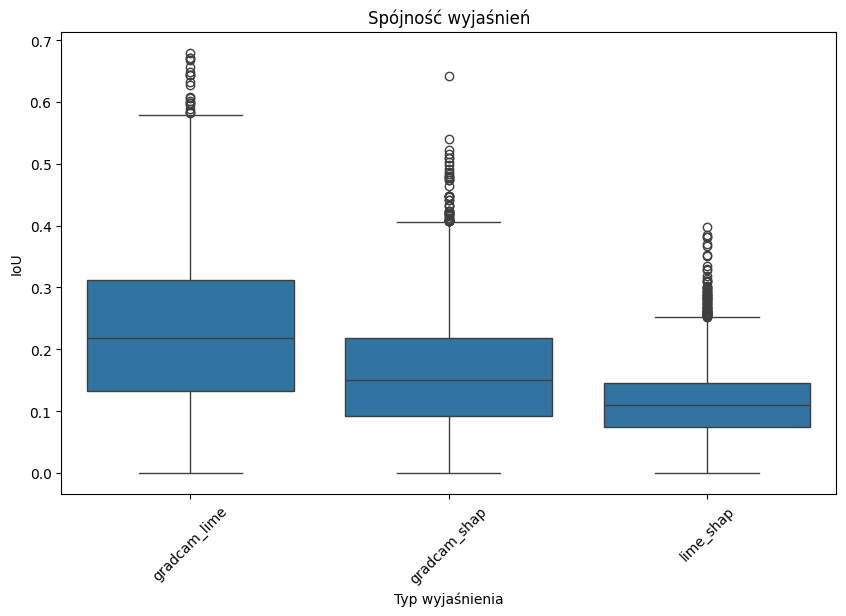
\includegraphics[width=.9\textwidth]{img/base_coherence}
	\caption{Spójność wyjaśnień}  \label{rys:base_coherence}
\end{figure}

\begin{table}[h]
	\centering
	\begin{tabular}{|c|c|}
		\hline
		\textbf{Metody XAI}     & \textbf{Średnie IoU} \\
		\hline
		\textbf{GradCAM i LIME} & 0.210750             \\
		\hline
		\textbf{GradCAM i SHAP} & 0.279382             \\
		\hline
		\textbf{LIME i SHAP}    & 0.113670             \\
		\hline
	\end{tabular}
	\caption{Średnie wartości IoU dla porównania spójności wyjaśnień}
	\label{tab:base_coherence}
\end{table}

Za pomocą wykresu pudełkowego (Rys \ref{rys:base_coherence}) przedstawione zostały wartości IoU dla porównania spójności wyjaśnień między różnymi metodami.
Natomiast Tabela \ref{tab:base_coherence} przedstawia porównanie spójności wyjaśnień między wybranymi metodami XAI, przy uzyciu średnich wartości IoU.

Wyniki pokazały, że największą spójnością wykazały się wyjaśnienia wygenerowane przez metody GradCAM i SHAP.
Natomiast najmniejszą spójność wykazały wyjaśnienia wygenerowane przez LIME i SHAP, co może wskazywać na różnice w podejściu tych metod do identyfikacji kluczowych cech.

Niska spójność między LIME i SHAP, pomimo wyższej spójności GradCAM i LIME oraz GradCAM i SHAP, może wskazywać na to, że obszary identyfikowane przez GradCAM są większe i bardziej ogólne.

GradCAM działa na poziomie cech wysokiego poziomu, które są identyfikowane na końcowych warstwach sieci neuronowej.
W związku z tym, GradCAM ma tendencję do zaznaczania większych regionów na obrazie, które zawierają kluczowe cechy wpływające na klasyfikację.
Dzięki temu wyjaśnienia generowane przez GradCAM są bardziej ogólne i obejmują szersze obszary obrazu.

LIME i SHAP z kolei, działają na bardziej szczegółowych poziomach.

W rezultacie, większe i bardziej ogólne regiony identyfikowane przez GradCAM mają większe szanse na nakładanie się z wyjaśnieniami LIME oraz SHAP.
Natomiast LIME i SHAP, ze względu na swoją szczegółowość, wykazują mniejszą spójność, ponieważ identyfikują bardziej precyzyjne i różniące się od siebie obszary.

\vspace{1cm}

W celu dokładniejszej analizy spójność wyjaśnień, wyniki podzielono ze względu na kategorie obrazów z bazy danych ImageNetS.
Analiza została przeprowadzona dla różnych kategorii obrazów.

\begin{figure}[h]
	\centering
	\begin{subfigure}[b]{0.3\textwidth}
		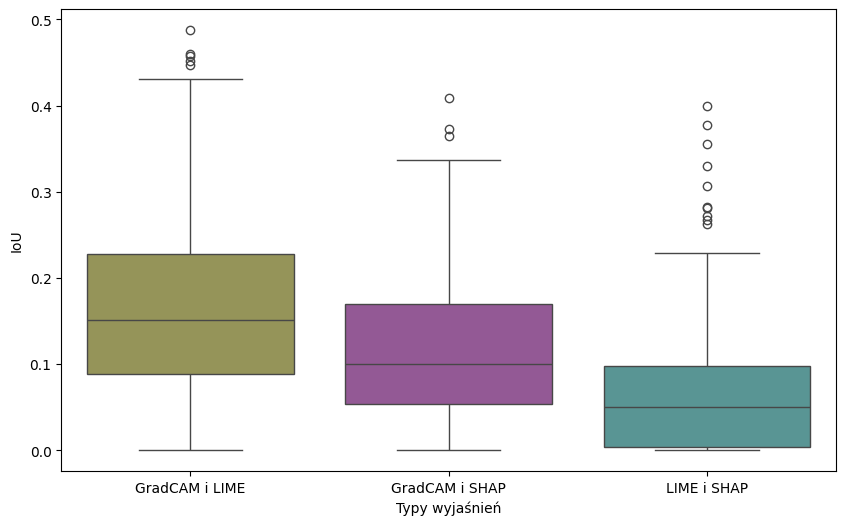
\includegraphics[width=.9\textwidth]{img/base_coherence_dog}
		\caption{\textbf{Dog}}  \label{}
	\end{subfigure}
	\begin{subfigure}[b]{0.3\textwidth}
		\centering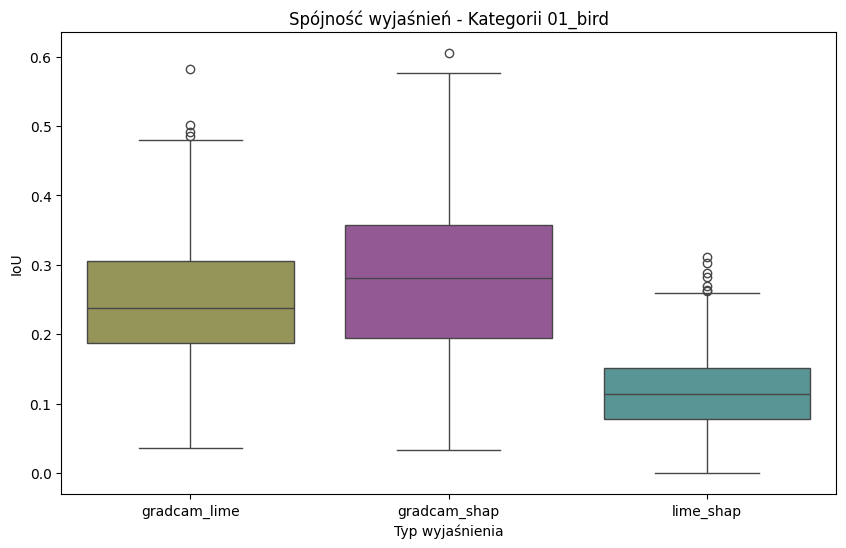
\includegraphics[width=.9\textwidth]{img/base_coherence_bird}
		\caption{\textbf{Bird}}  \label{}
	\end{subfigure}
	\begin{subfigure}[b]{0.3\textwidth}
		\centering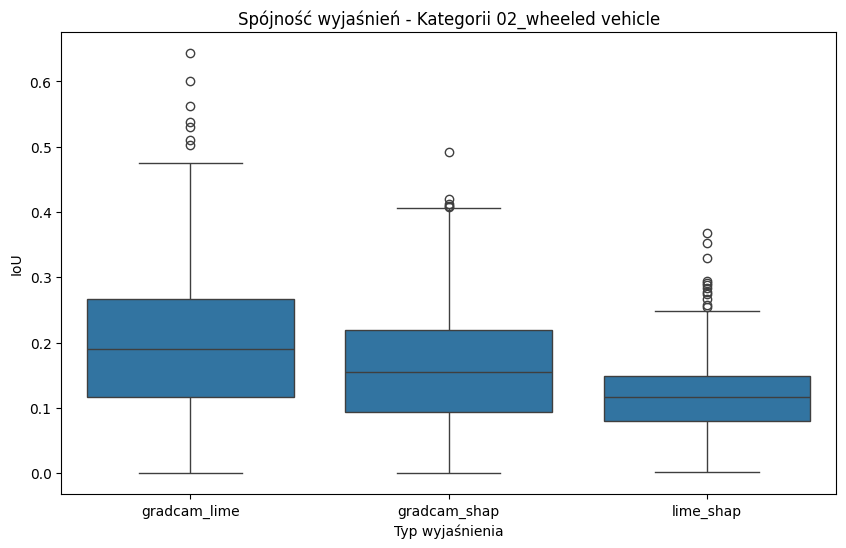
\includegraphics[width=.9\textwidth]{img/base_coherence_vehicle}
		\caption{\textbf{Vehicle}}  \label{}
	\end{subfigure}
	\begin{subfigure}[b]{0.3\textwidth}
		\centering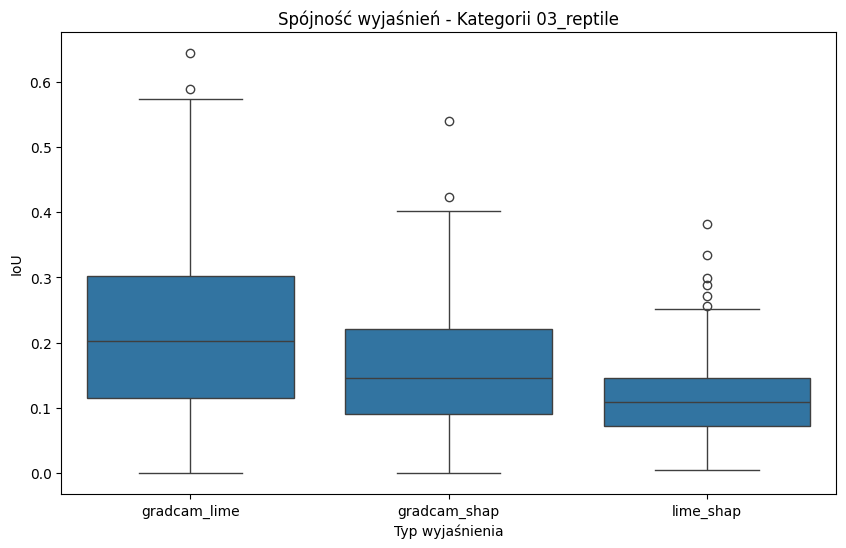
\includegraphics[width=.9\textwidth]{img/base_coherence_reptile}
		\caption{\textbf{Reptile}}  \label{}
	\end{subfigure}
	\begin{subfigure}[b]{0.3\textwidth}
		\centering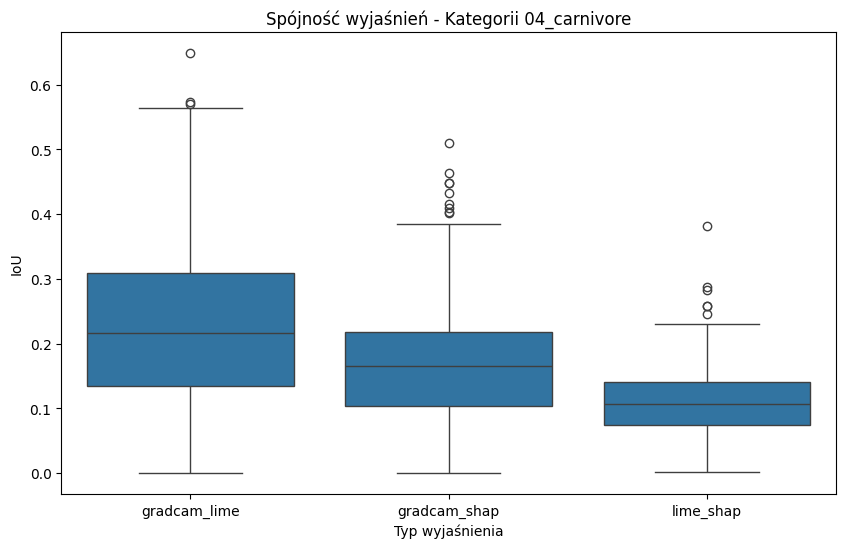
\includegraphics[width=.9\textwidth]{img/base_coherence_carnivore}
		\caption{\textbf{Carnivore}}  \label{}
	\end{subfigure}
	\begin{subfigure}[b]{0.3\textwidth}
		\centering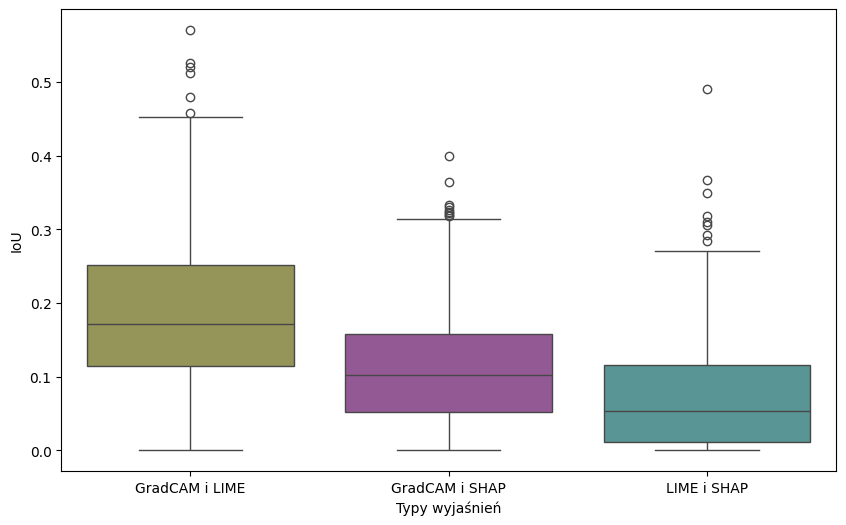
\includegraphics[width=.9\textwidth]{img/base_coherence_insect}
		\caption{\textbf{Insect}}  \label{}
	\end{subfigure}
	\begin{subfigure}[b]{0.3\textwidth}
		\centering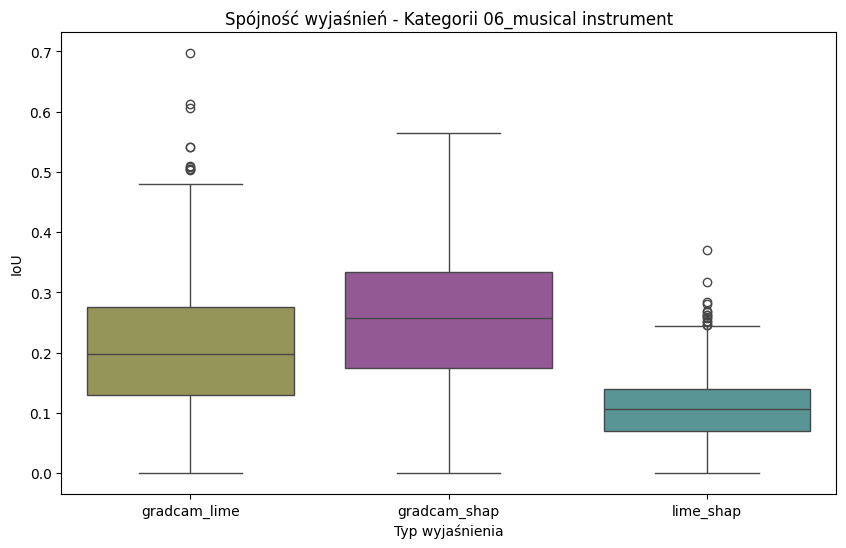
\includegraphics[width=.9\textwidth]{img/base_coherence_music}
		\caption{\textbf{Instrument}}  \label{}
	\end{subfigure}
	\begin{subfigure}[b]{0.3\textwidth}
		\centering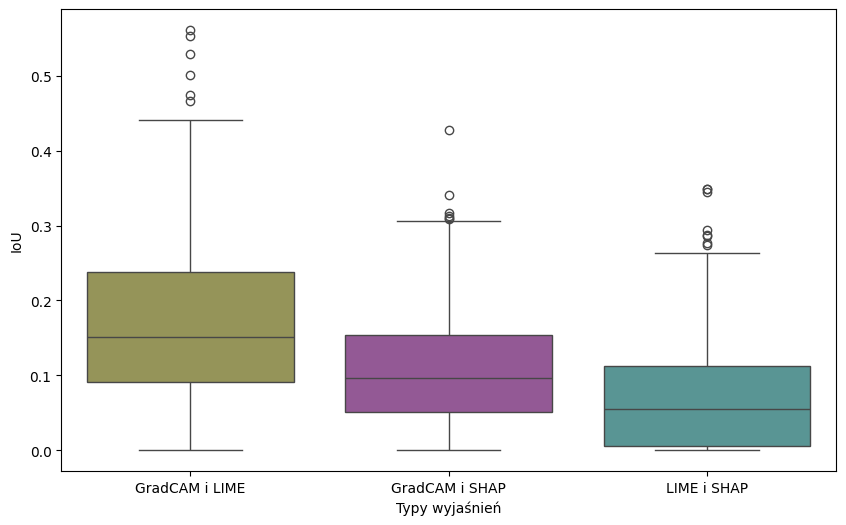
\includegraphics[width=.9\textwidth]{img/base_coherence_primate}
		\caption{\textbf{Primate}}  \label{}
	\end{subfigure}
	\begin{subfigure}[b]{0.3\textwidth}
		\centering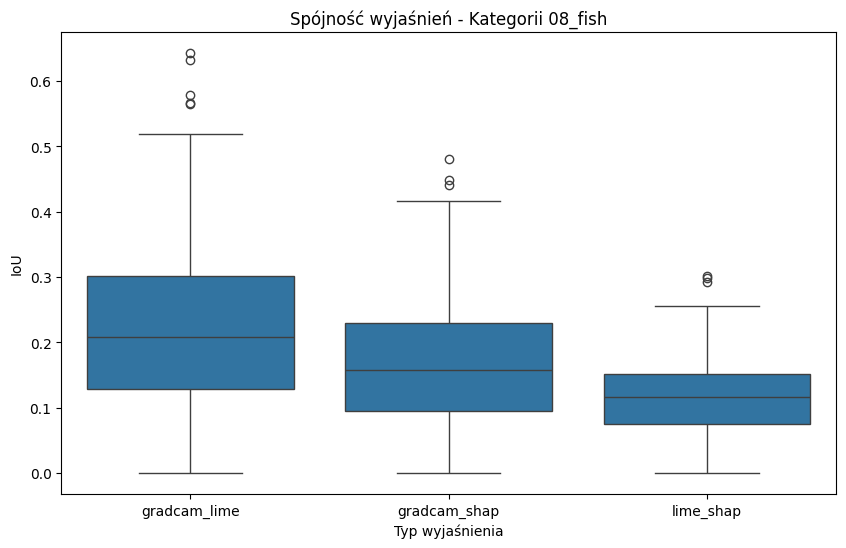
\includegraphics[width=.9\textwidth]{img/base_coherence_fish}
		\caption{\textbf{Fish}}  \label{}
	\end{subfigure}
	\caption{Spójność wyjaśnień dla różnych kategorii}
	\label{rys:coherence_category}
\end{figure}

\begin{table}[h]
	\centering
	\begin{tabular}{|c|c|c|c|}
		\hline
		\textbf{Kategoria}           & \textbf{GradCAM i LIME} & \textbf{GradCAM i SHAP} & \textbf{LIME i SHAP} \\
		\hline
		\textbf{Pies}                & 0.206546                & 0.277394                & 0.111613             \\
		\hline
		\textbf{Ptak}                & 0.247909                & 0.277716                & 0.117751             \\
		\hline
		\textbf{Pojazd na kołach}    & 0.204956                & 0.283621                & 0.118001             \\
		\hline
		\textbf{Gad}                 & 0.191600                & 0.287120                & 0.113589             \\
		\hline
		\textbf{Mięsorzerca}         & 0.196739                & 0.292880                & 0.110058             \\
		\hline
		\textbf{Insekt}              & 0.235127                & 0.273465                & 0.119031             \\
		\hline
		\textbf{Instrument muzyczny} & 0.208132                & 0.253540                & 0.109638             \\
		\hline
		\textbf{Naczelny}            & 0.195163                & 0.283483                & 0.105888             \\
		\hline
		\textbf{Ryba}                & 0.210879                & 0.285220                & 0.117462             \\
		\hline
	\end{tabular}
	\caption{Średnie wartości IoU dla różnych kategorii}
	\label{tab:base_coherence_categories}
\end{table}

Dane zostały przedstawione w ten sam sposób jak wcześniej, za pomocą wykresu (Rys \ref{rys:coherence_category}) oraz tabeli (Tabela \ref{tab:base_coherence_categories}) przedstawiającej średnie wartości IoU w celu prównania spójności w zależności od kategorii obrazu.

Spójność LIME i SHAP jest podobna dla wszystkich kategorii obrazów, przy czym najgorsza jest dla kategorii Naczelny, natomiast najlepsza dla kategorii Insect.
Spójność między tymi dwoma metodami jest najgorsza niezależnie od kategorii.

Spójność GradCAM i LIME jest różna w zależności od kategorii obrazów, przy czym najgorsza jest dla kategorii Gad, natomiast najlepsza dla kategorii Ptak i Insekt.
Spójność między tymi dwiema metodami nigdy nie jest najlepsza ani najgorsza niezależnie od kategorii.

Spójność GradCAM i SHAP jest różna w zależności od kategorii obrazów, przy czym najgorsza jest dla kategorii Instrument muzyczny, natomiast najlepsza dla Mięsorzerca.
Spójność miedzy tymi dwiema metodami zawsze jest najlepsza nie zależnie od kategorii.

\vspace{1cm}
W celu zweryfikowania czy wielkość wyjaśnień miała znaczenie przeanalizowano spójność wyjaśnień podzieloną ze względu na wielkość obiektów na obrazie.

\begin{figure}[h]
	\centering
	\begin{subfigure}[b]{0.3\textwidth}
		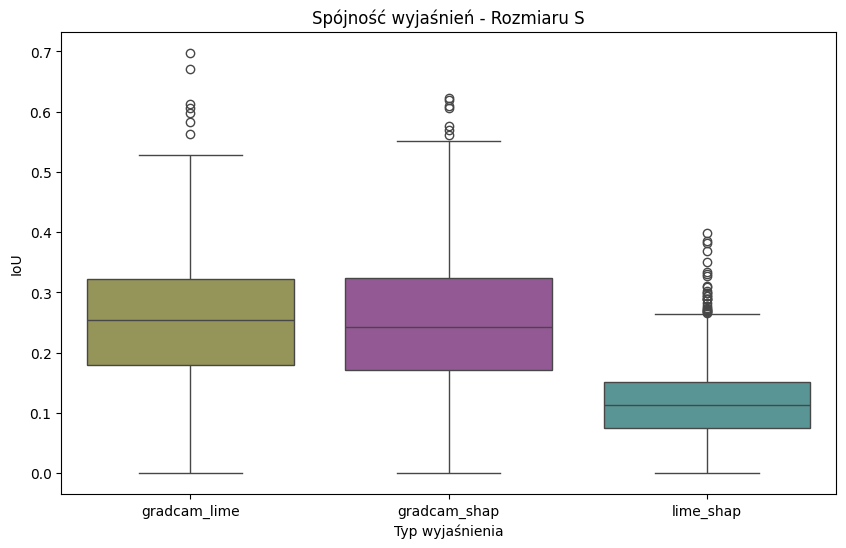
\includegraphics[width=1\textwidth]{img/base_coherence_size_S}
		\caption{Mały obiekt}  \label{}
	\end{subfigure}
	\begin{subfigure}[b]{0.3\textwidth}
		\centering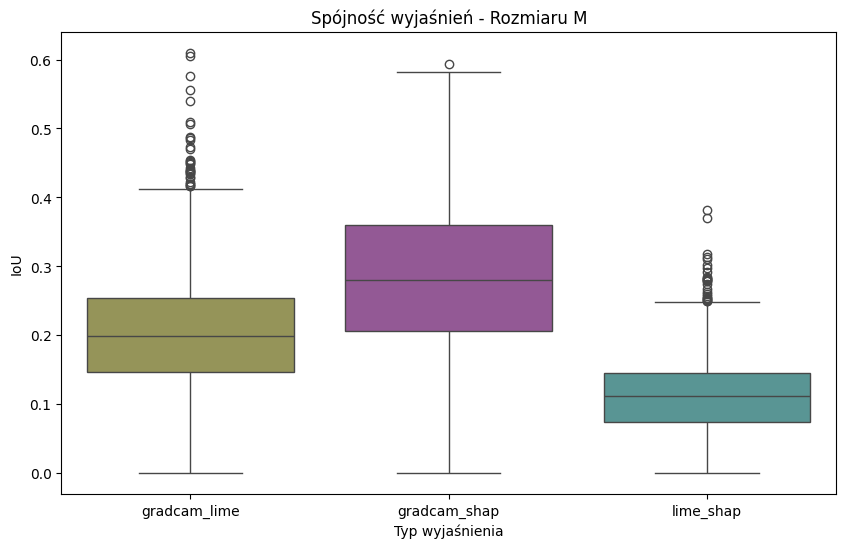
\includegraphics[width=1\textwidth]{img/base_coherence_size_M}
		\caption{Średni obiekt}  \label{}
	\end{subfigure}
	\begin{subfigure}[b]{0.3\textwidth}
		\centering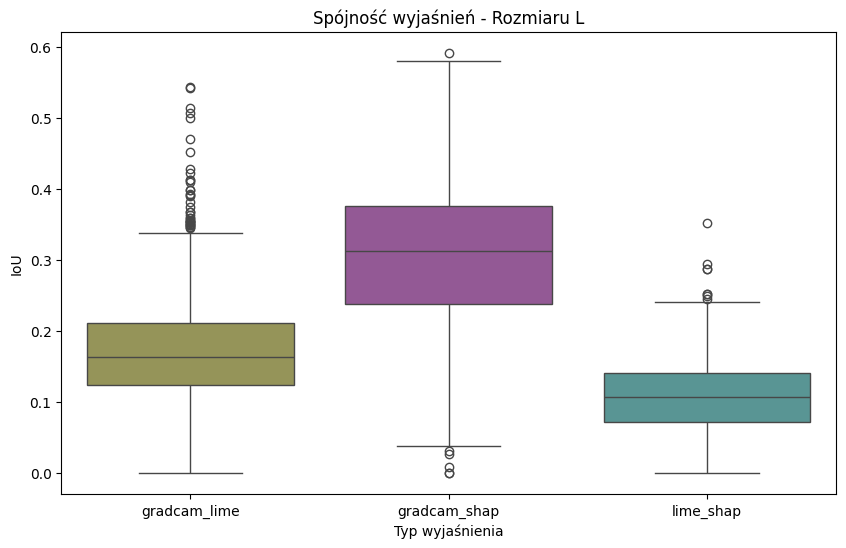
\includegraphics[width=1\textwidth]{img/base_coherence_size_L}
		\caption{Duży obiekt}  \label{}
	\end{subfigure}
	\caption{Spójność wyjaśnień dla różnych rozmiarów obiektów}
	\label{rys:coherence_size}
\end{figure}

\begin{table}[h]
	\centering
	\begin{tabular}{|c|c|c|c|}
		\hline
		\textbf{Rozmiar} & \textbf{GradCAM vs LIME} & \textbf{GradCAM vs SHAP} & \textbf{LIME vs SHAP} \\
		\hline
		\textbf{Mały}    & 0.253597                 & 0.250014                 & 0.117247              \\
		\hline
		\textbf{Średni}  & 0.204279                 & 0.282094                 & 0.114313              \\
		\hline
		\textbf{Duży}    & 0.172506                 & 0.307551                 & 0.109135              \\
		\hline
	\end{tabular}
	\caption{Średnie wartości IoU dla różnych rozmiarów}
	\label{tab:base_coherence_size}
\end{table}

Tak jak w poprzednich przypadkach wyniki przedstawiono na wykresie (Rys \ref{rys:coherence_size}) oraz tabeli (Tabela \ref{tab:base_coherence_size}) przedstawiającej średnie wartości IoU dla porównania spójności wyjaśnień w zależności od rozmiaru obiektu na obrazie.

Wyniki:
\begin{itemize}
	\item \textbf{Obiekty małe} - Największa spójność wyjaśnień występuje między metodami GradCAM i LIME oraz GradCAM i SHAP.
	      Spójność między LIME i SHAP jest znacznie niższa tak jak w poprzednich analizach.
	\item \textbf{Obiekty średnie} - GradCAM i SHAP ponownie wykazują największą spójność, następnie GradCAM i LIME, a najniższą spójność odnotowano między LIME i SHAP.
	\item \textbf{Obiekty duże} - Spójność wyjaśnień między GradCAM i SHAP jest najwyższa. GradCAM i LIME mają niższą spójność, a najniższą spójność obserwuje się między LIME i SHAP.
\end{itemize}

Dodatkowo zauważono, że spójność między GradCAM i LIME była odwrotnie proporcjonalna do wielkości obiektu.
Im mniejeszy obiekt, tym większa była spójność między tymi metodami.
Podobny trend zaobserwowano w przypadku spójności między LIME i SHAP, choć wpływ wielkości obiektu był mniejszy.
Natomiast spójność między GradCAM i SHAP była proporcjonalnie zależna od wielkośći.
Im większy obiekt, tym większa była spójność między tymi metodami.

Warto zauważyć, że metody takie jak LIME i SHAP są wrażliwe na dobór parametrów.
Te zależności od parametrów mogą wpływać na stabilność i spójność wyjaśnień generowanych przez te techniki.
Co może częściowo może tłumaczyć podobne wyniki między LIME i SHAP niezależnie od rozmiaru obiektu.

